\subsubsection{まとめ}
\paragraph{問題は何だったのか?}
結局、問題は何だったのかといえば、
特急券予約システムのクレジットカードによる決済のモデルが考慮不足だったということになる。

まず、おサイフケータイのクレジットカードを変更すると、
特急券予約システムを新規に契約せねばならず、
予約会員証も新規に作成しなければならない。

しかし、変更前の予約を行った古いクレジットカードは、
その予約の特急券を受け取るときに必要になる。
何故なら、クラス図\ref{fig:ExpressReservationClassDiagram}で見るように、
個々の予約を表す特急券予約システムからクレジットカードにリンクが設定されているからである。

\begin{figure}[h]
	\centering
	{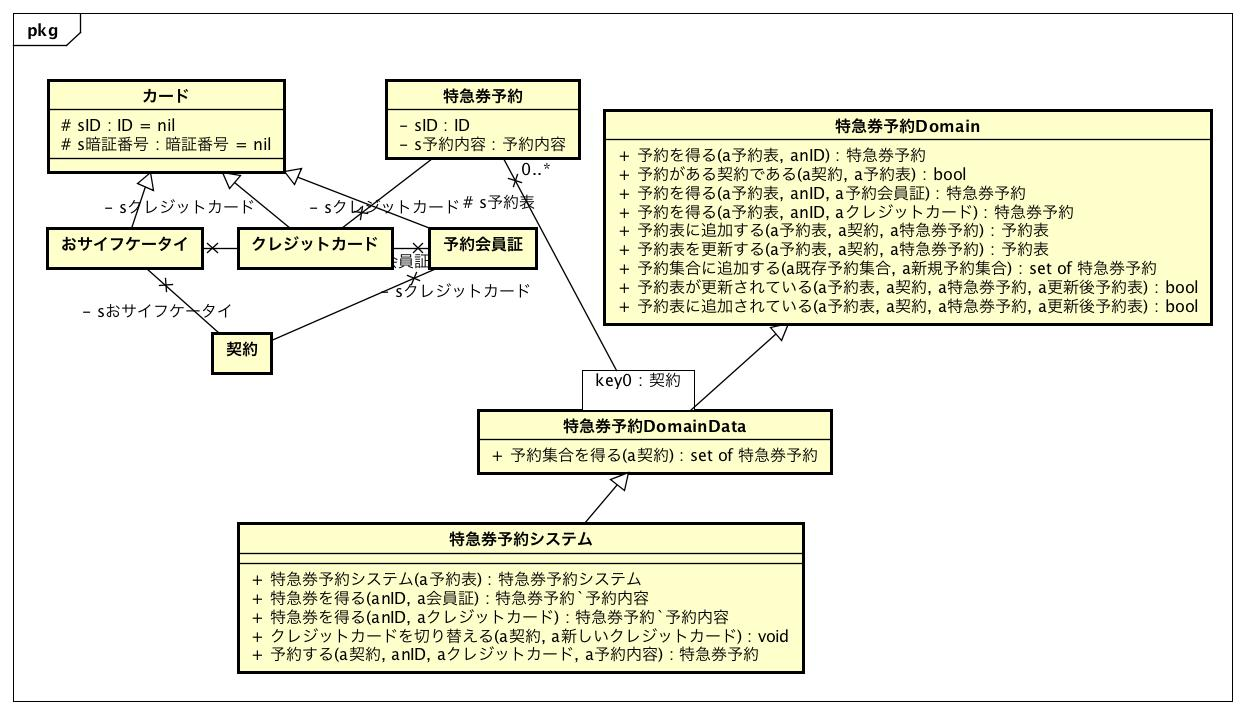
\includegraphics[width=55zw, keepaspectratio]{./image/ClassDiagram.jpg}}
	\caption{クラス図(特急券予約システム)}
	\label{fig:ExpressReservationClassDiagram}
	\index{くらすすとっきゅうけんよやくしすてむ@クラス図(特急券予約システム)}
\end{figure}

このような構造でも、変更後にすべての特急券予約システムからクレジットカードへのリンクを
新しいクレジットカードに変更していれば問題はないはずだが、
恐らく、変更に掛かる効率を理由に、古いクレジットカードとリンクしたままになっているのであろう。
設計上の理由で、ユーザーに迷惑を掛ける仕様となっている訳である。

さらに、モデルに問題があった。
予約会員証は新規に作るのが普通であるが、
クレジットカード会社の都合による変更のため、
新規に契約する費用は無料となった。
そのため、予約会員証は古いものを使用することになった。
契約は新規だが、予約会員証は古く、
そしてクラス図\ref{fig:ExpressReservationClassDiagram}から分かるように、
予約会員証からリンクしているクレジットカードは、
変更前の古いものであるという訳である。

これではまずいと思って、鉄道会社Aの係員がリンクされているクレジットカードを新しいものにしたようである。
その結果、変更前の特急券予約システムを予約会員証で特急券を得ることができなかった。


\paragraph{本来どうすべきだったのか?}
本来、特急券予約システムは契約\footnote{口座と言ってもよいが、本モデルでは契約という名前にした}
とリンクが設定されているべきであり、
契約がクレジットカードとリンクしているべきである。

予約会員証も契約を介してクレジットカードを参照できるようにすべきである。

このようにしておけば、契約に変更があっても、古い特急券予約システムは新しい契約を介して、新しいクレジットカードにアクセスでき、
同じく予約会員証も新しいクレジットカードにアクセスできる。

本来どうすべきだったのかを検証するVDM++モデルは、1日で記述および検証ができた。

詳細は、「特急券予約システムシステムの問題点を推測し、修正した仕様」を参照のこと。


\paragraph{統計情報}
注釈抜きのVDM++ソース行数は、492行、
モデル作成工数は約1日、発表用の資料作成とVDM++モデルの読みやすさのための整形・清書に約2日かかった。

なお、上記モデルの作成工数は、筆者が問題を解決するために消費した工数より少ない。